\section{Intrinsic filtering for 2D manifold surface}

\begin{figure*}[htb]
\centering
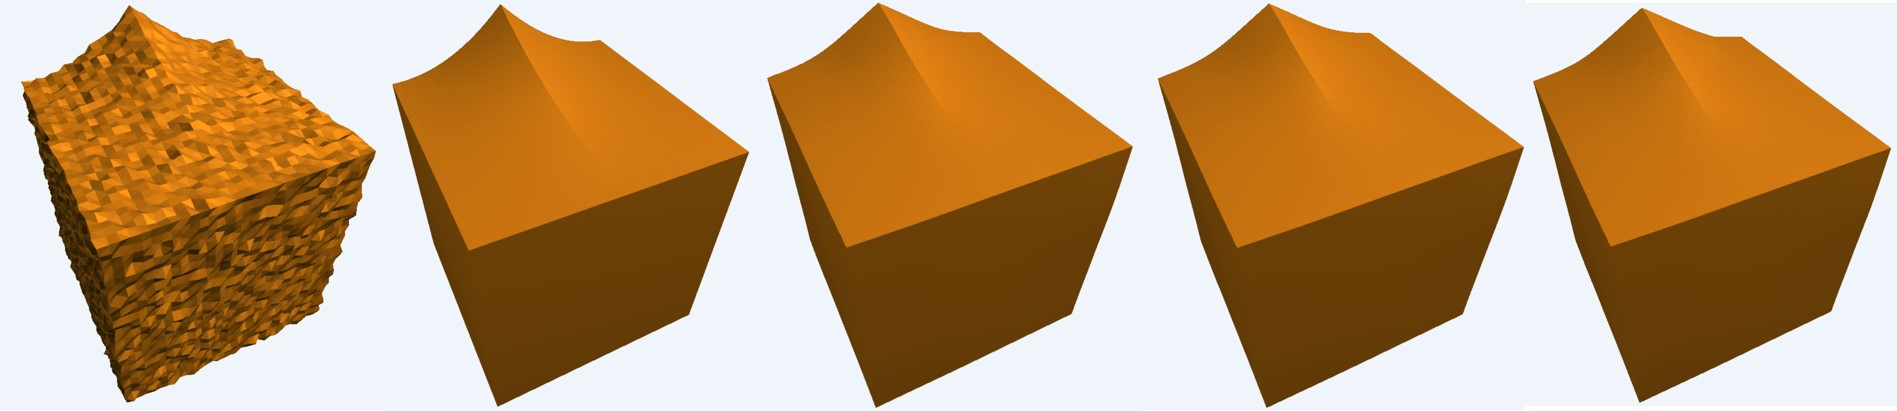
\includegraphics[width = 15.0cm]{results/norm.jpg}
\vspace{0.5mm}
\caption{ The results of different conditions (or change 0.3 noise?).}
\label{Fig:norm}
\end{figure*}

In this section, we introduce our intrinsic filtering framework for 2D manifold surfaces in detail.
Furthermore, we explain that those classical filtering methods can be viewed as a simplification basing ours.

\subsection{Filtering for 2D manifold surface}

Suppose we are interested in signals that are defined on 2D manifold surface $\Omega$ with values in domain $\Gamma$,
the filtered output signal $\bar{J_p}$ at point $p$ can be produced by this general form
\begin{equation}
\begin{aligned}
\label{Eq:GeneralForm}
\bar{J_{p}} = \frac{1}{W_{p}}\int_{\mathcal{N}(p)}\omega_{p, q}J_{q}d_{q}\, ,
\end{aligned}
\end{equation}
where $J_{q}$ denotes the value of the signal at point $q$; $\mathcal{N}(p)$ is the neighborhood of the point $p$;
$\omega_{p, q}$ indicates the weight for each neighboring signal,
and $W_{p} = \int_{\mathcal{N}(p)}\omega_{p, q}d_{q}$ is the normalization factor for ensuring the sum of all $\omega_{p,q}$ equal to 1.
The construction of $\omega_{p,q}$ is very important, it directly relates to the performance of edge-preserving.

Here, we give the following weight which reflects the cumulative difference of input signal:
\begin{equation}
\begin{aligned}
\label{Eq:IntrinsicWeight}
\omega_{p,q} = g(d^{s}(\varphi_{p}, \varphi_{q}); \sigma_{s})g(d^{r}(\psi_p, \psi_q); \sigma_{r})\, ,
\end{aligned}
\end{equation}
where $g(\cdot \,; \cdot)$ is Gaussian function, $\sigma_{s}$, $\sigma_{r}$ are variance parameters and the function $d^s$ and $d^r$ are defined as:
 \begin{equation}
 \begin{aligned}
 \label{Eq:IntrinsicDistance}
 d^{s}(\varphi_p, \varphi_q) = (\int_{L}||\varphi_{q_{i+1}} - \varphi_{q_i}||^{n}ds\,\,)^{1/n}\, ,
 \\
 d^{r}(\psi_p, \psi_q) = (\int_{L}||\psi_{q_i} - \psi_{p}||^{m}ds\,\,)^{1/m}\, .
 %\sqrt{\sum\limits_{x,x+1\in\phi}||I_{x+1}-I_{x}}\, ,
 \end{aligned}
 \end{equation}

Note that $L$ is the geodesic path connecting points $p$ and $q$.
$\varphi$ and $\psi$ can represent different signal values, for example position, Gaussian curvature and normal on a 2D manifold surface.
$q_{i+1}$ and $q_i$ are adjacent points in path $L$.

The cumulative difference of input signal can reflect the local structure of desired signal.
The main reason is that we consider the difference not only between adjacent signals but also start-end signals.
According to different problems, we can choose suitable parameters $\varphi$, $\psi$, $n$ and $m$.

Equation \ref{Eq:IntrinsicDistance} which reflects the similar distance between signals can be approximated as:
 \begin{small}
 \begin{equation}
 \begin{aligned}
 \label{Eq:IntrinsicDiscreteDist}
 d^{s}(\varphi_p, \varphi_q) = (\sum_{q_{i+1}, q_i \in{L}}|\!|\varphi_{q_{i+1}} - \varphi_{q_i}|\!|^{n}|\!|q_{i+1} - q_{i}|\!|\,)^{1/n}\, ,
 \\
 d^{r}(\psi_p, \psi_q) = (\sum_{q_{i+1}, q_i \in{L}}|\!|\psi_{q_i} - \psi_{p}|\!|^{m}|\!|q_{i+1} - q_{i}|\!|\,)^{1/m}\, .
 \end{aligned}
 \end{equation}
 \end{small}

As image is a special 2D manifold,
the geodesic filtering \cite{grazzini2009edge} and propagation filtering \cite{Chang2015propagated} which are widely used in image can be thought of a special value by our method.
We think about the 4-neighbor connecting in image, so this form is $||q_{i+1} - q_{i}|| = 1$ in a geodesic path $L$.
Geodesic filtering \cite{grazzini2009edge} only uses cumulative difference in adjacent image signals during filtering process.
Namely, when $n=2$, the image intensity value $I$ as a signal value $\varphi$ and $d^{r}(\psi_p, \psi_q) == 1$,
our intrinsic filtering is simplified, gets the similar distance between intensities of geodesic image filtering:
 \begin{equation}
 \begin{aligned}
 \label{Eq:GeodesicDistance}
 d^{s}(I_p,I_q) = (\sum_{q_{i+1}, q_i \in{L}}||I_{q_{i+1}} - I_{q_i}||^{2}\,)^{1/2}\, .
 %\sqrt{\sum\limits_{x,x+1\in\phi}||I_{x+1}-I_{x}}\, ,
 \end{aligned}
 \end{equation}

In a similar way, our intrinsic filtering is simplified as a propagation image filtering by $n=2$, $m=2$, $\varphi$ and $\psi$ both represent the image intensity.
Therefore,
 \begin{equation}
 \begin{aligned}
 \label{Eq:PropagationDistance}
 d^{s}(I_p, I_q) = (\sum_{q_{i+1}, q_i \in{L}}||I_{q_{i+1}} - I_{q_i}||^{2}\,)^{1/2}\, ,
 \\
 d^{r}(I_p, I_q) = (\sum_{{q_i} \in{L}})||I_{q_i} - I_p||^2\,)^{1/2}\, .
 \end{aligned}
 \end{equation}

In addition, our approach is equivalent to the promotion of bilateral filtering.
As is known to all, the classical nonlinear bilateral filtering uses two Gaussian functions as the spatial and range weights respectively:
\begin{equation}
\begin{aligned}
\label{Eq:BilateralWeight}
\omega_{p,q} = g(d(p, q); \sigma_{s})g(d(\psi_p, \psi_q); \sigma_{r})\, ,
\end{aligned}
\end{equation}
where,
\begin{equation}
\begin{aligned}
\label{Eq:BilateralDistance}
d(p, q) = ||p - q||\, ,
\\
d(\psi_{p}, \psi_{q}) = || \psi_{p} - \psi_{q} ||\, .
\end{aligned}
\end{equation}

 As the ability of Gaussian function, the filtered signal $J_{p}$ is influenced by the neighborhood only if their spatial and range distances are enough closed.
 As a result, the bilateral filter is able to smooth the signal while preserve the edge structures.
 The effectiveness of bilateral filter relies on the range function which reflects the local information of signal, and then applies the averaging weights as the filtered output.
 However, the difference between the input signal values $J_{p}$ and $J_{q}$ can not provides reliable prediction for that between the desired signal values $\bar{J_{p}}$ and $\bar{J_{q}}$.

Our intrinsic filtering build a relation between $p$ and $q$, which providing more reliable information about the structure of the desired output.
This relation can be depicted in Figure \ref{Fig:relation}.
Our method inherits the advantage of bilateral filter and become more adaptive to context of signal.

\begin{figure*}[htb]
\centering
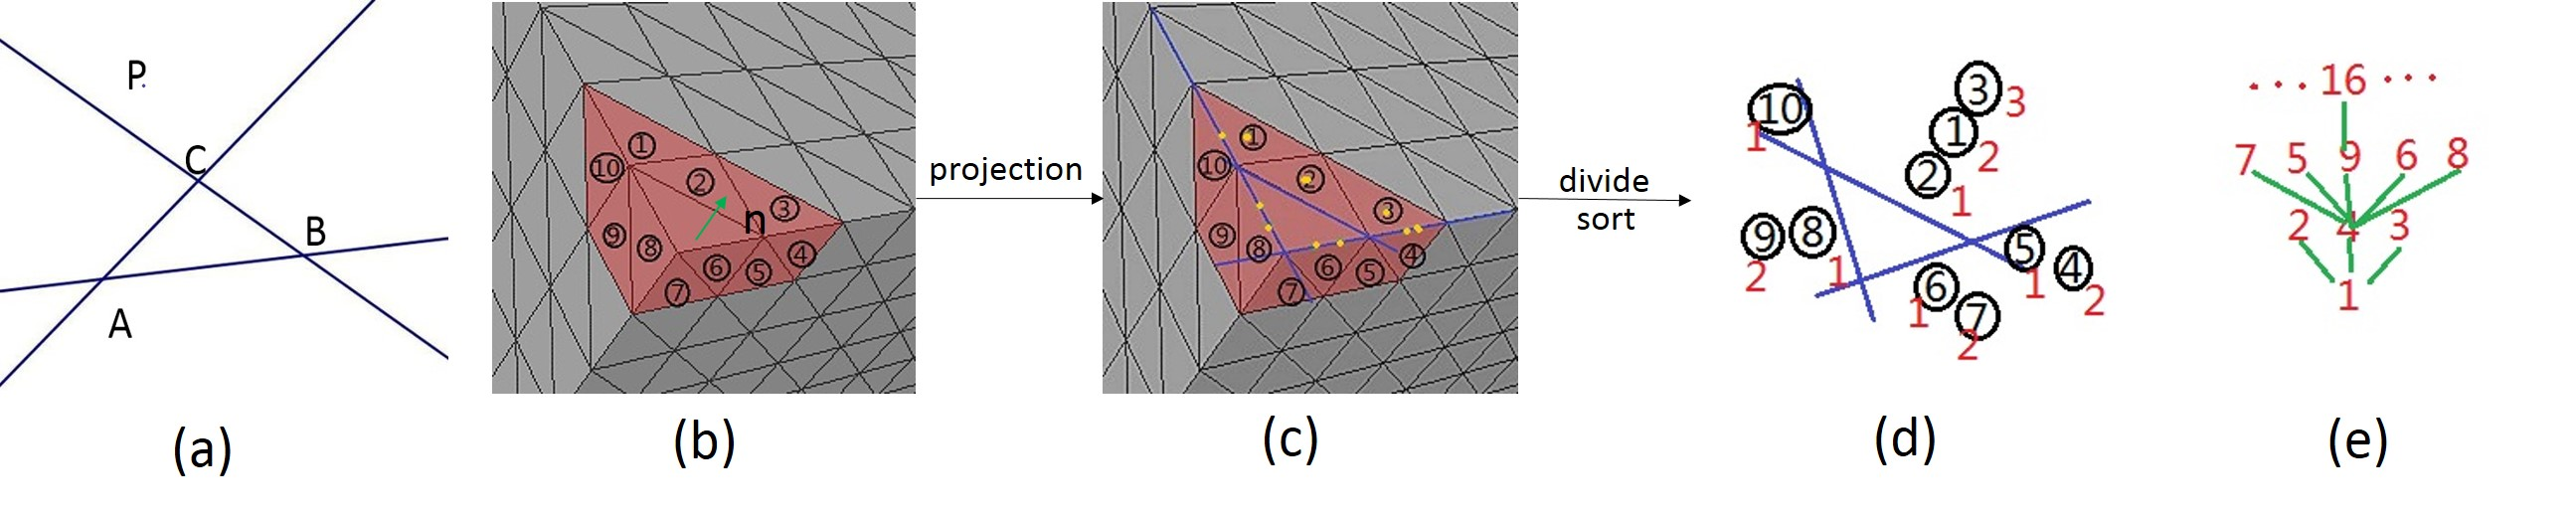
\includegraphics[width = 15.0cm]{results/path.jpg}
\vspace{-3mm}
\caption{ The process of generation path.}
\label{Fig:path}
\end{figure*}

\subsection{Filtering mesh geometry}

Given a noisy triangle mesh, our goal is to filter the noise while less change the mesh structure.
In order to achieve this purpose, we adapt a two-stage process which be widely used in mesh filtering.
Firstly, noisy face normals are filtered iteratively by equation~\ref{Eq:IntrinsicMeshFiltering}.
Secondly, according to the filtered face normals, vertex positions are updated iteratively though gradient descent.

{\bfseries Filtering face normals.}
When we consider normals as a surface signal defined over the original triangle mesh, it is easy to put the intrinsic filtering algorithm to mesh denoising.
For a triangle face $f_{i}$, its outward normal $\mathbf{n_{i}}$ can be calculated by outer product easily.
Then we consider $\mathbf{n_{i}}$ as a signal associated with the face centroid $c_{i}$.
In order to filter the face normals $\mathbf{n_{i}}$, we need find a path $L$ to connect $\mathbf{n_{i}}$ and its neighborhood $\mathbf{n_{j}}$.
Then a filtered face normal $\bar{\mathbf{n_{i}}}$ is computed from our intrinsic mesh filtering:
 \begin{equation}
 \begin{aligned}
 \label{Eq:IntrinsicMeshFiltering}
 \bar{\mathbf{n_{i}}} = \frac{1}{W_{i}}\sum_{\mathclap{f_{j}\in\mathcal{N}_{i}}}A_{j}g(d^{s}(\mathbf{n_{i}}, \mathbf{n_{j}}); \sigma_{s})g(d^{r}(\mathbf{n_{i}}, \mathbf{n_{j}}); \sigma_{r})\mathbf{n_{j}}\, .
 \end{aligned}
 \end{equation}
  here,
 \begin{equation}
 \begin{aligned}
 \label{eq:IntrinsicMeshDistance}
 d^{s}(\mathbf{n_{i}}, \mathbf{n_{j}}) = (\sum_{x, x+1\in{L}}||\mathbf{n_{x+1}}-\mathbf{n_{x}}||^{n}\,\,)^{1/n}\, ,
 \\
 d^{r}(\mathbf{n_{i}}, \mathbf{n_{j}}) = (\sum_{x\in{L}}||\mathbf{n_{x}}-\mathbf{n_{i}}||^{m}\,\,)^{1/m}\, ,
 \end{aligned}
 \end{equation}
where $W_{i}$ is the normalization factor,
calculated by
$||\sum\limits_{\mathclap{f_{j}\in\mathcal{N}_{i}}}A_{j}g(d^{a}(\mathbf{n_{i}}, \mathbf{n_{j}}); \sigma_{s})g(d^{r}(\mathbf{n_{i}}, \mathbf{n_{j}}); \sigma_{r})||$
which ensures that $\bar{\mathbf{n_{i}}}$ is a unit normal;
$A_j$ is the area of face $f_j$;
$\mathcal{N}_{i}$ is the neighborhood of face $f_{i}$.
In our paper, we use the geometrical neighborhood, defined at the paper~\cite{Zhang2015Filter}.

Note that equation \ref{Eq:IntrinsicMeshFiltering} can be derived from equation \ref{Eq:GeneralForm}.
The reason that $A_j$ existing is accumulation of infinitesimal area because the domain of integration is triangle face.
Furthermore, we give up the distance between adjacent centroid of triangle faces to facilitate the calculation in equation \ref{eq:IntrinsicMeshDistance}.

Although the geodesic algorithm gives the shortest distance $d^s$ and $d^r$, it is computationally expensive and difficult to implement algorithm.
Considering the shortcomings, we introduce a simple, fast and effective pattern for choosing paths which is shown in Section \ref{Sec:path}.
We find that this operation is about an order of magnitude faster than applying shortest path in obtaining similar results.
Furthermore, the filter results that applying the particular paths often have better power on dealing with some details, like edges and corners from the figure \ref{Fig:norm}.
And for triangle mesh, we conduct the experiment in the presence of $m$ and $n$ taking different values.
We find that $m=1$ and $n=1$ can obtain the best results because feature structure is sparse in triangle mesh.
These are also shown in the figure \ref{Fig:norm}.

 {\bfseries Updating vertices.} After all face normals is filtered, the vertex positions need to be updated to cater to these new normals.
 We adopt the iterative scheme in the paper~\cite{sun2007fast} to update the vertex positions.
 Namely, for a face $f_{i}$, we calculate its updated vertex positions via the following iteration form
 \begin{equation}
 \begin{aligned}
 \label{vertexupdate}
 %\mathclap include sum �±�
 \bar{v_{i}}^{(t+1)} = \bar{v_{i}}^{(t)} + \frac{1}{|{\mathcal{F}_{i}}|}\sum_{j\in\mathcal{F}_{i}}\mathbf{\bar{n}_{j}}[\mathbf{\bar{n}_{j}}\cdot(\bar{c_{j}}^{(t)}-\bar{v_{j}}^{(t)})]\, ,
 \end{aligned}
 \end{equation}
 where $\bar{v_{j}}^{(t)}$ is the value of $\bar{v_{i}}$ in the $t-th$ iteration,
 $\mathcal{F}_{i}$ is the index set of the incident faces for $\bar{v_{i}}$,
 $|\cdot|$ denotes the cardinality of a set,
 and $\bar{c_{j}}^{(t)} = \sum_{i=1}^{3}\bar{v_{j_{i}}}^{(t)}/3$ is the centroid of the triangle $f_{j}$.
 This scheme is actually based on the orthogonality between the normal and the three edges of each face on the mesh.
 Then adopts a gradient descend process for solving that orthogonality equation in the conditions of  $L_2$ error.

 In our experiments, 10 to 20 iterations are sufficient for achieving satisfactory results and approximately up to above conditions.
 Our filtered process is summarized in Algorithm~\ref{alg:1}.
 In the next section, we introduce a simple but effective method for selecting a particular pattern for our propagated mesh filtering.


\begin{algorithm}\caption{Propagation mesh filtering framework}
\label{alg:1}
\begin{algorithmic}
\STATE {\textbf{Input:} Initial mesh $M_{in}$, number of iterations $k_{iter}$.}
\STATE{\textbf{Output:} Filtered mesh $M_{out}$.}
\STATE{1: $M^{(0)} = M_{in}$}
\STATE{2: \textbf{for} $s = 1$ to $k_{iter}$ \textbf{do}}
\STATE{3: ~~~Compute face normals {$n_i$} of mesh $M^{(s-1)}$;}
\STATE{4: ~~~Get pathes from {$\mathcal{N}_i$} to {$n_i$} according to section \ref{Sec:path};}
\STATE{5: ~~~Compute filtered normals {$\mathbf{\bar{n_i}}$} according to~\ref{Eq:IntrinsicMeshFiltering};}
\STATE{6: ~~~Compute updated mesh $M^{(s)}$ according to {$\mathbf{\bar{n_i}}$};}
\STATE{7: \textbf{end for}}
\STATE{8: $M_{out} = M^{k_{iter}}$.}
\end{algorithmic}
\end{algorithm}

 \section{Path chosen for mesh filtering}
 \label{Sec:path}


%Fig.~\ref{fig:example} for an example
\begin{figure*}
\centering
\subfigure[]
{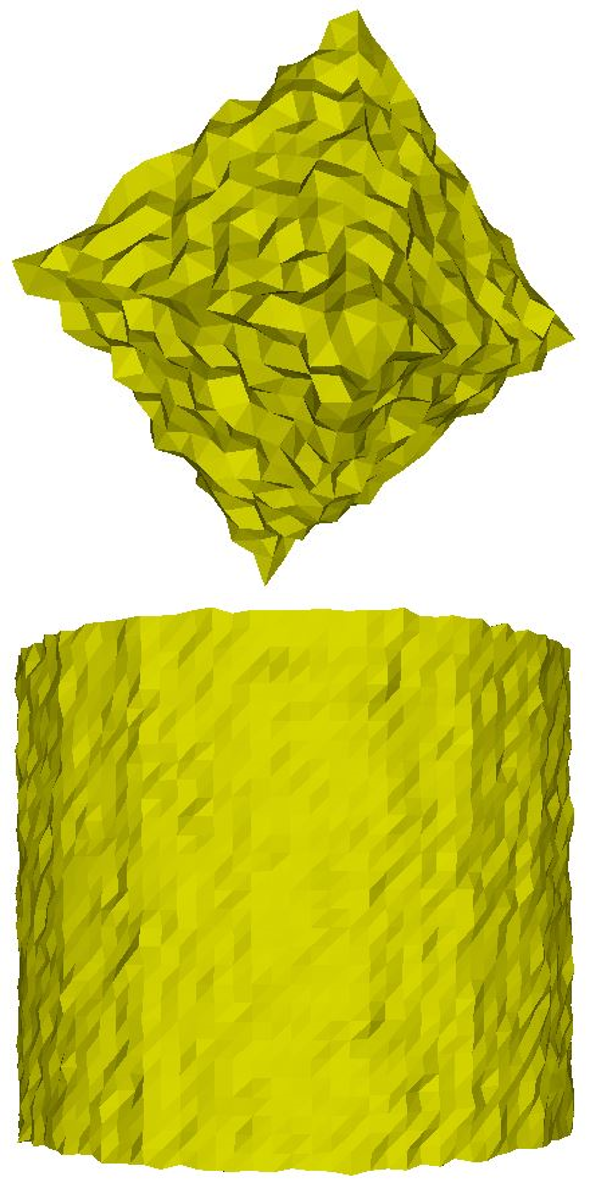
\includegraphics[width = 1.8cm]{results/oct_prism_Noisy.png}}%4.0cm two ��
\subfigure[]
{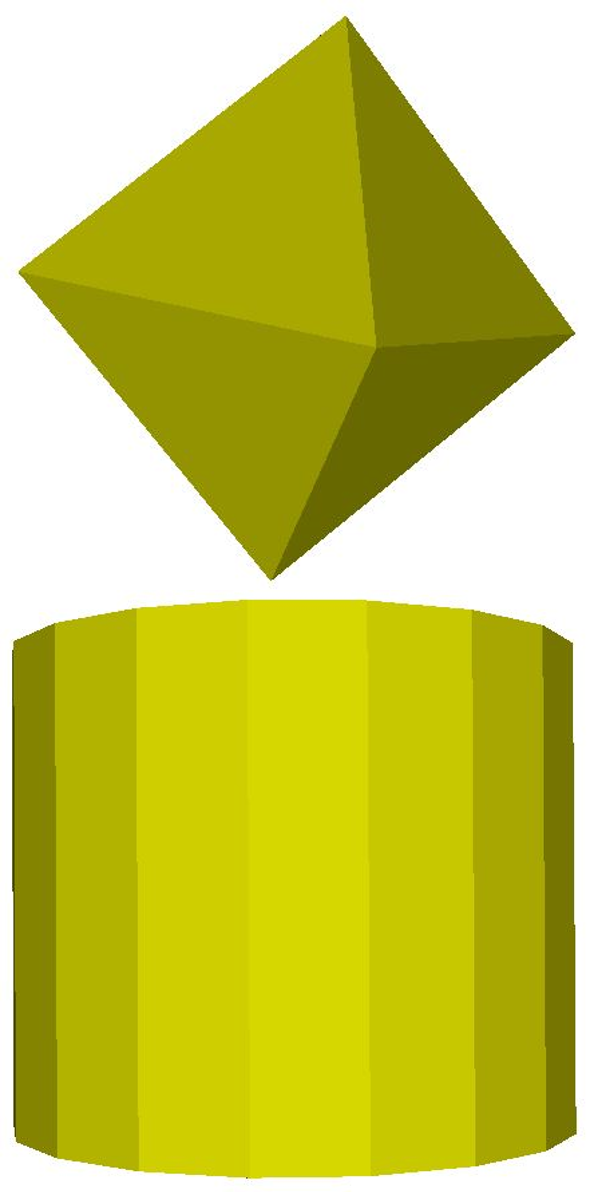
\includegraphics[width = 1.8cm]{results/oct_prism_Original.png}}
\subfigure[]
{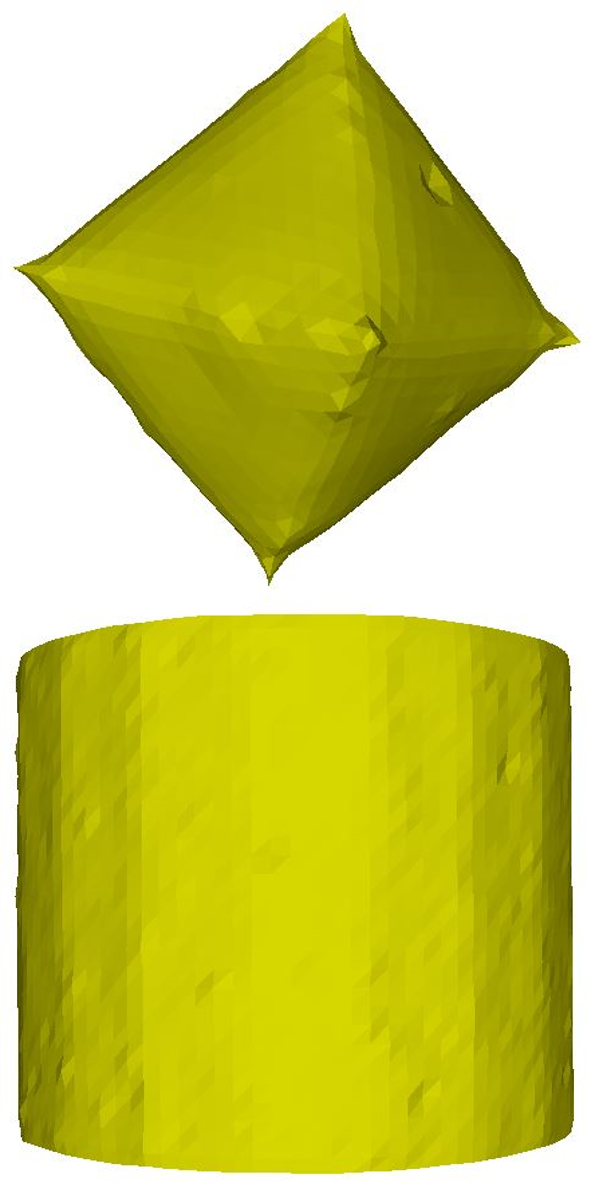
\includegraphics[width = 1.8cm]{results/oct_prism_FDCO03.png}}
\subfigure[]
{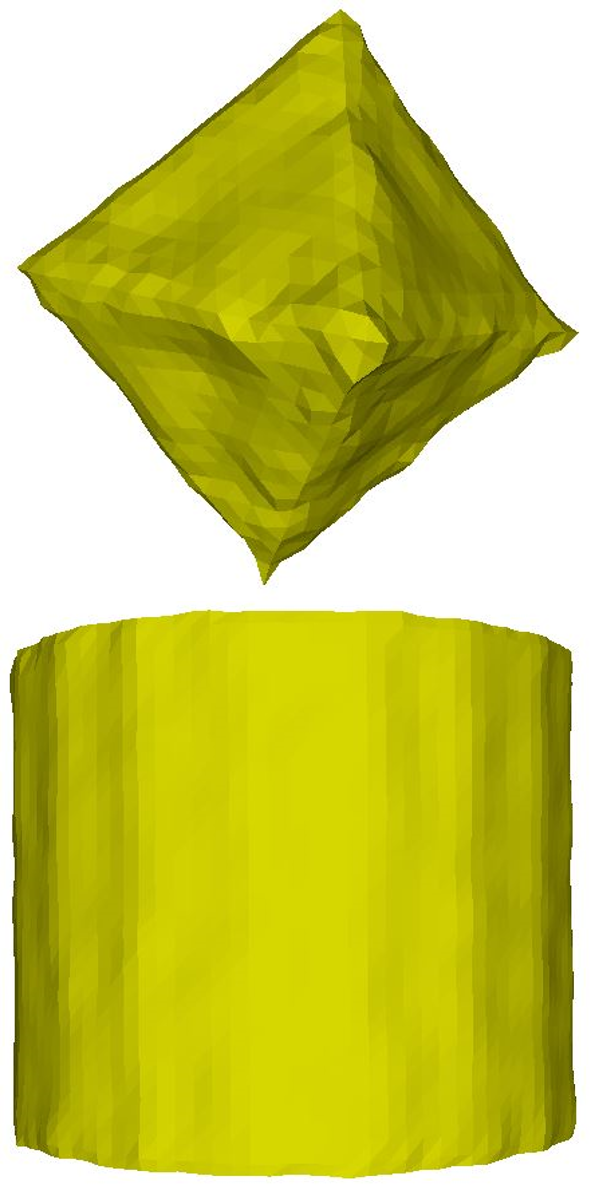
\includegraphics[width = 1.8cm]{results/oct_prism_JDD03.png}}
\subfigure[]
{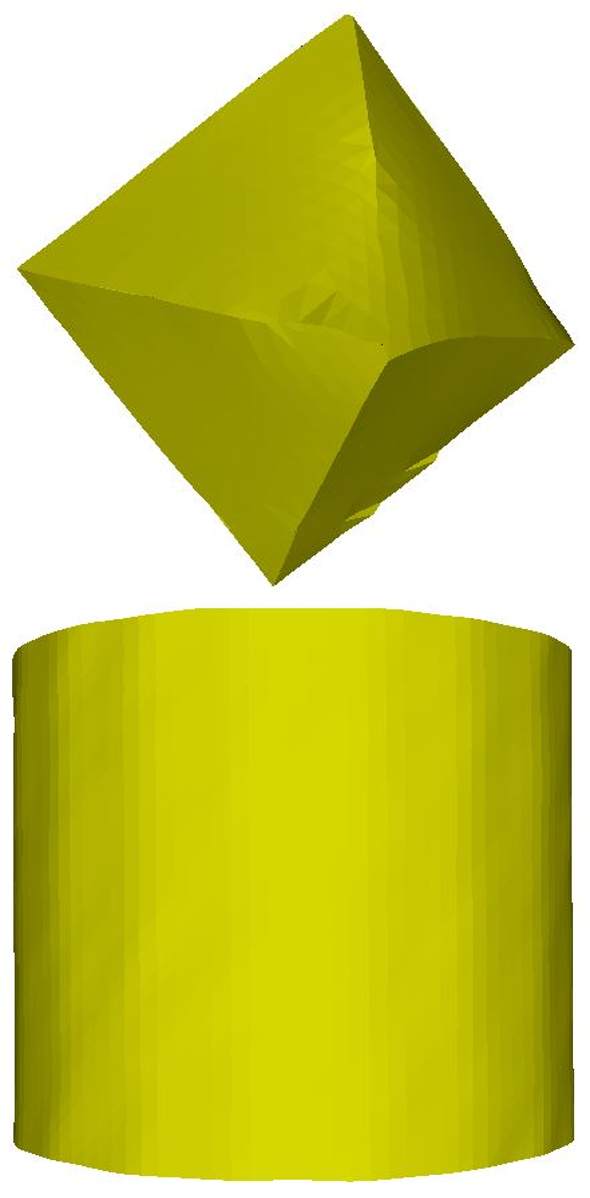
\includegraphics[width = 1.8cm]{results/oct_prism_SRML07.png}}
\subfigure[]
{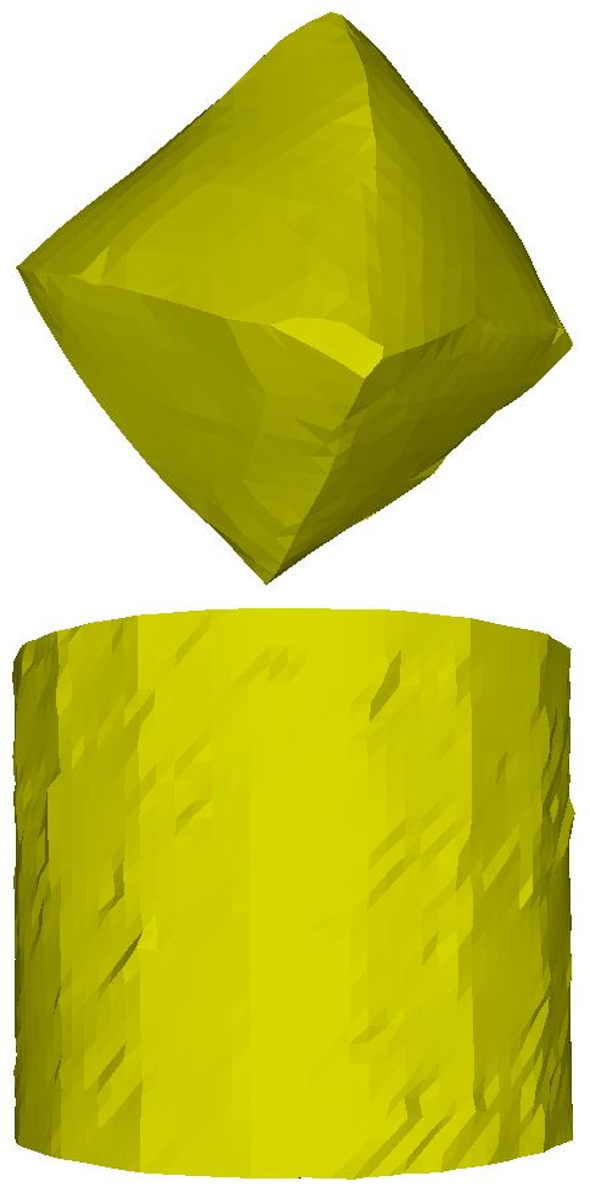
\includegraphics[width = 1.8cm]{results/oct_prism_ZFAT11local.png}}
\subfigure[]
{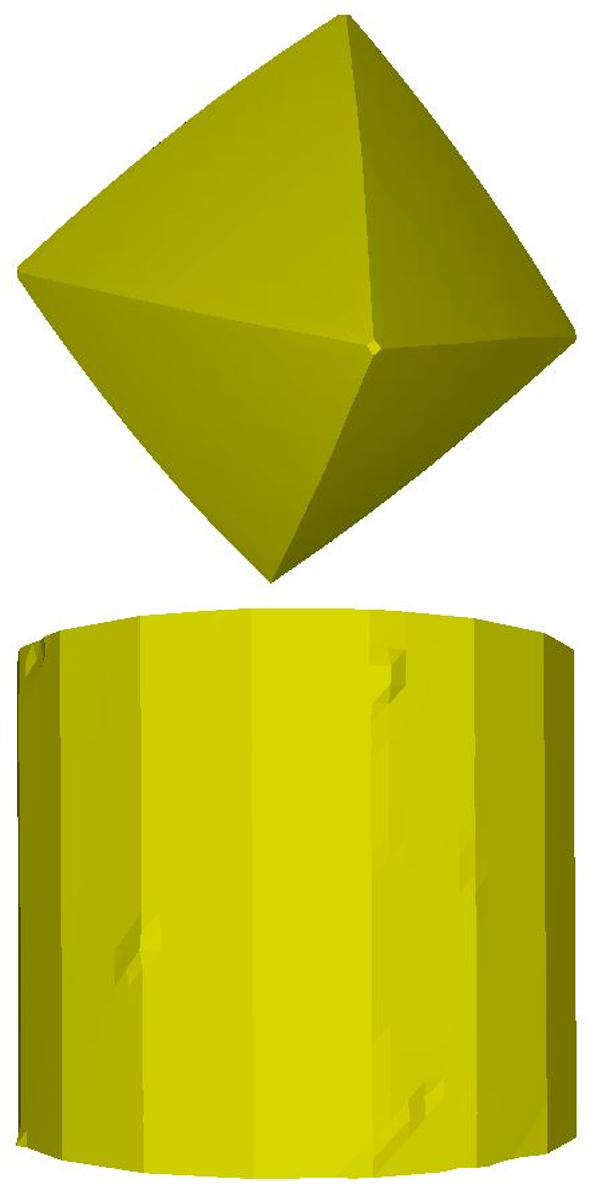
\includegraphics[width = 1.8cm]{results/oct_prism_HS13.png}}
\subfigure[]
{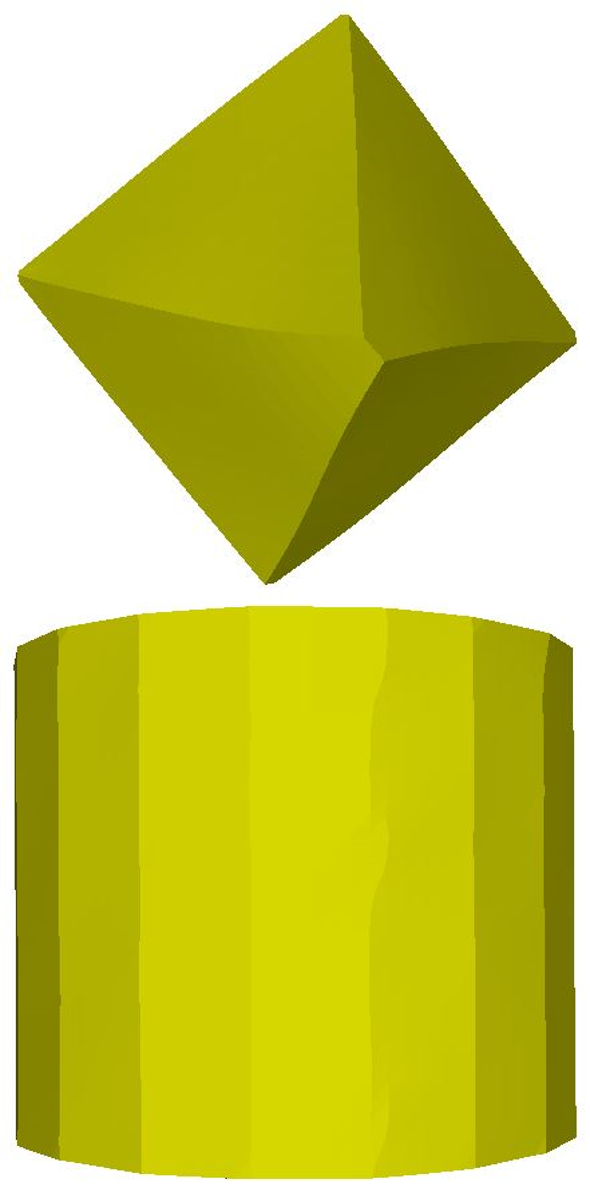
\includegraphics[width = 1.8cm]{results/oct_prism_PG15.png}}
\subfigure[]
{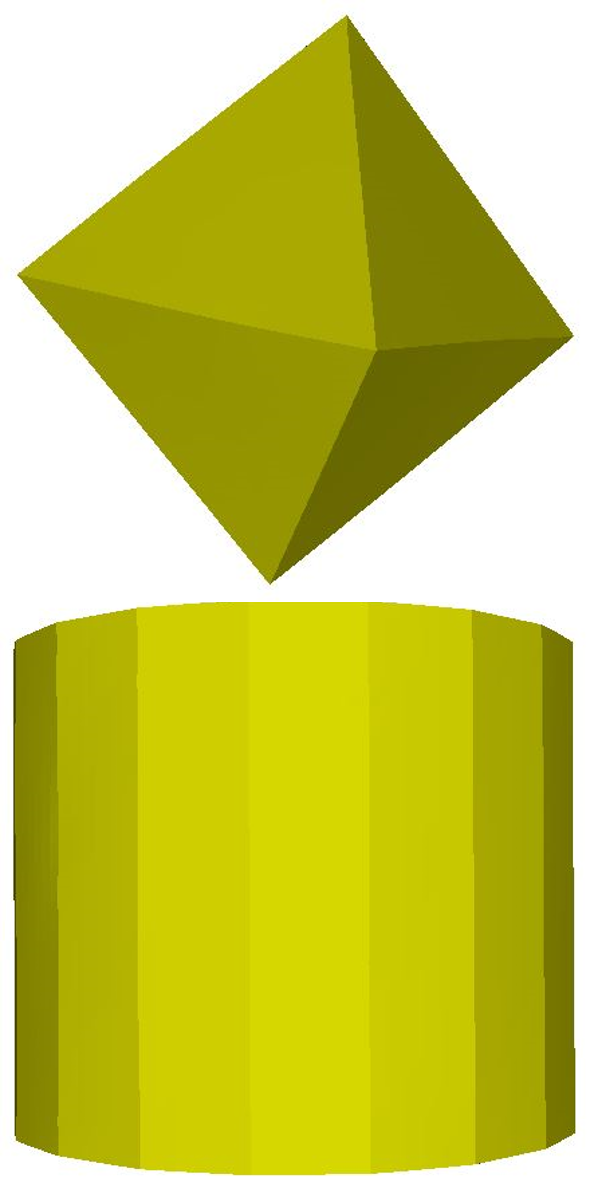
\includegraphics[width = 1.8cm]{results/oct_prism_our.png}}
%\subfigure[ֱ�ӱ��ⲻ��Ҫ��ʾ] {\includegraphics[height=2in,width=2in,angle=-90]{results/IMG_3164_small/img_result.jpg}}
\caption{ Comparisons with other methods on synthetic meshes. One with sharp corners and the other with weak edges. (a) The noisy mesh( Gaussian noise, $\sigma_E = 0.3$ ). (b) The original mesh.
(c-i) The results of Fleishman et al~\cite{fleishman2003bilateral},
Jones et al~\cite{jones2003non}, Sun et al~\cite{sun2007fast}, Zheng et al~\cite{zheng2011bilateral}(l), He et al~\cite{he2013mesh}, Zhang et al~\cite{Zhang2015Filter} and our result separately.}
\label{Fig:oct_prism}
\end{figure*}

%%Fig.~\ref{fig:example} for an example
%\begin{figure*}
%\centering
%\subfigure[]
%{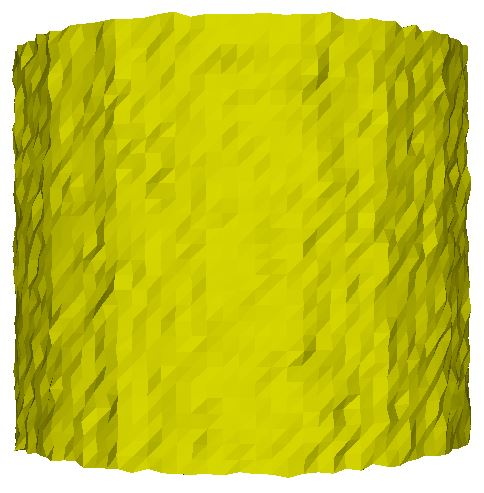
\includegraphics[width = 1.8cm]{results/prism_Noisy.jpg}}%4.0cm two ��
%\subfigure[]
%{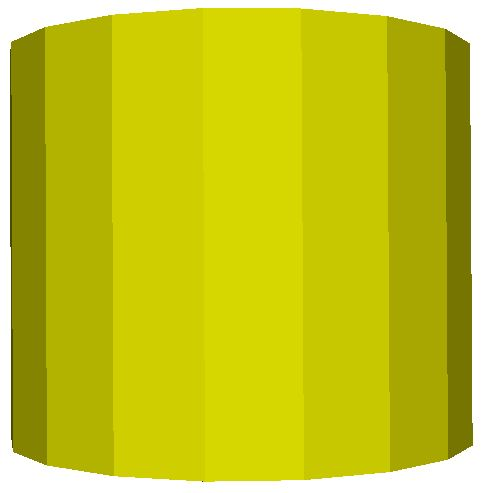
\includegraphics[width = 1.8cm]{results/prism_Original.jpg}}
%\subfigure[]
%{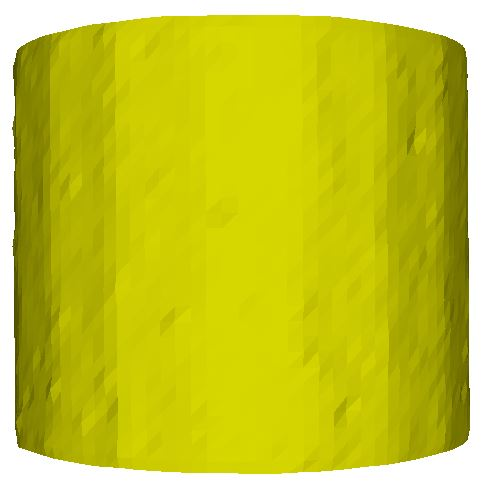
\includegraphics[width = 1.8cm]{results/prism_FDCO03.jpg}}
%\subfigure[]
%{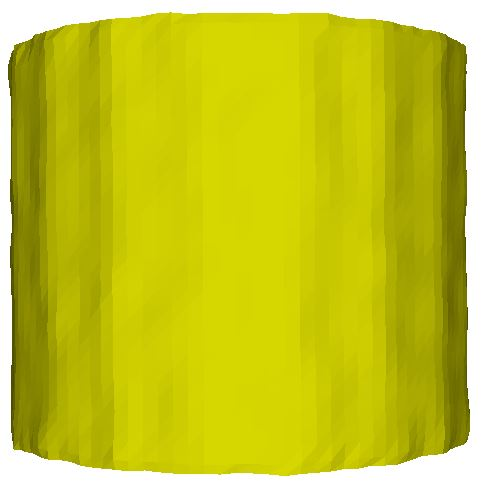
\includegraphics[width = 1.8cm]{results/prism_JDD03.jpg}}
%\subfigure[]
%{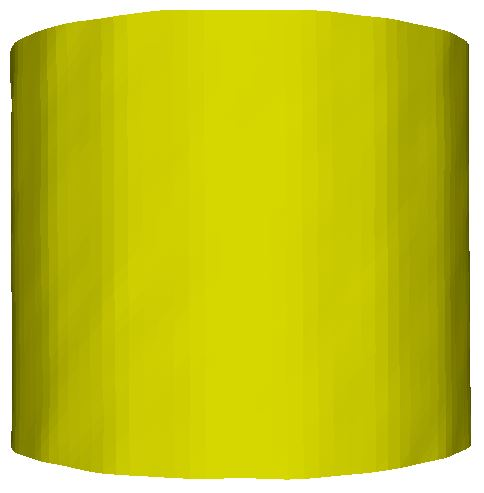
\includegraphics[width = 1.8cm]{results/prism_SRML07.jpg}}
%\subfigure[]
%{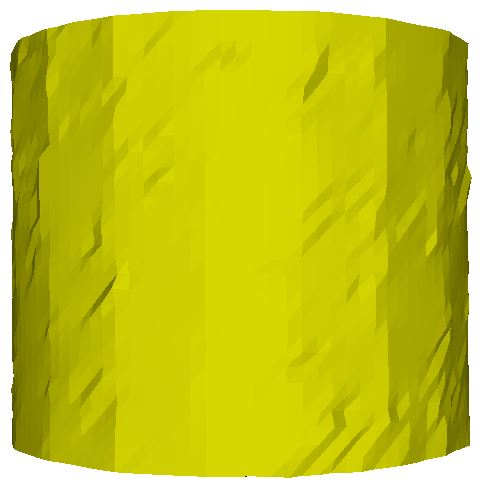
\includegraphics[width = 1.8cm]{results/prism_ZFAT11local.jpg}}
%\subfigure[]
%{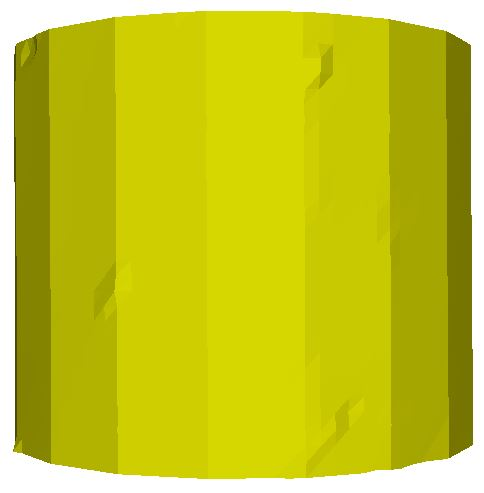
\includegraphics[width = 1.8cm]{results/prism_HS13.jpg}}
%\subfigure[]
%{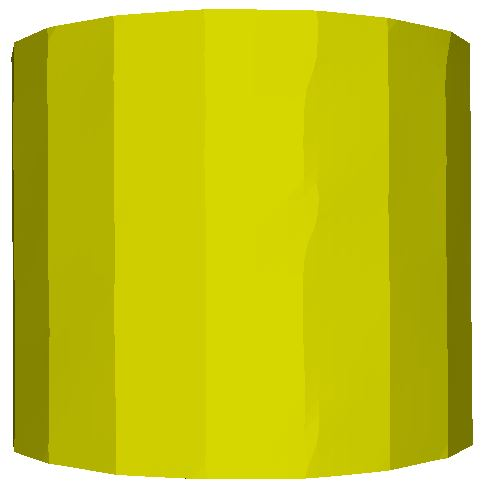
\includegraphics[width = 1.8cm]{results/prism_PG15.jpg}}
%\subfigure[]
%{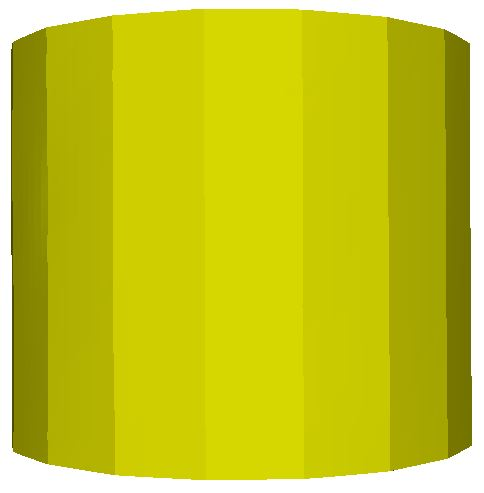
\includegraphics[width = 1.8cm]{results/prism_our.jpg}}
%%\subfigure[ֱ�ӱ��ⲻ��Ҫ��ʾ] {\includegraphics[height=2in,width=2in,angle=-90]{results/IMG_3164_small/img_result.jpg}}
%\caption{ Comparisons with other methods on a synthetic mesh with weak edges. (a) The noisy mesh( Gaussian noise, $\sigma_E = 0.1$ ). (b) The original mesh.
%(c-i) The results of Fleishman et al~\cite{fleishman2003bilateral},
%Jones et al~\cite{jones2003non}, Sun et al~\cite{sun2007fast}, Zheng et al~\cite{zheng2011bilateral}(l), He et al~\cite{he2013mesh}, Zhang et al~\cite{Zhang2015Filter} and our result separately.}
%\label{Fig:weakEdge}
%\end{figure*}

 In image, many particular patterns can be chosen for generating the path because of the regular coordination.
 These patterns are simple and easy to be thought about.
 But in triangle mesh, it is very difficult to obtain a good pattern that preserves the mesh feature for giving pathes.
 The easiest way to be thought of is that applying the shortest path algorithm on the triangle mesh.
 However, figure \ref{Fig:norm} shows this method is time consuming.
 We deal with this problem in this paper within the context of mesh denoising.

 Our method is based on the following theory: the areal coordinates of triangle segments the plane into seven regions.
 Areal coordinates are extremely useful in engineering applications involving triangular subdomains.
 These make analytic integrals often easier to evaluate, and Gaussian quadrature tables are often presented in terms of area coordinates.
 In the context of a triangle, the areal coordinates of a point $P$ are equivalent to the ratios of the areas of $PBC$, $PCA$ and $PAB$ to the area of the reference triangle $ABC$,
 shown in the figure~\ref{Fig:path}(a).
 Because the ratios are a plus or a minus, it divide the plane where the triangle is to seven parts.
 That gives us an approach to obtain a particular pattern solving the problem of paths.

 Thus for each triangle $f_i$, we can projective its neighborhood $\mathcal{N}_i$ to the plane where $f_i$ is.
 In more detail, we only projective their centroid to that plane.
 Then based on the three points of $f_i$, we divide these centroid to seven parts.
 Note that, if the projection point of one triangle centroid falls into the face $f_i$, we throw it away from $\mathcal{N}_i$.
 In this way, we give each neighbor a label that belong to a specified region.
 %And in some extend, these regions can depict the local structure of a mesh.
 After that, we sort these neighbors belong to the same region basing their face centroid distance to $c_i$ in original noisy mesh.
 Finally, we provide a particular pattern to assign the path for matching the ordered neighbors.
 The entire process is depicted in the figure~\ref{Fig:path}.

 From the figure~\ref{Fig:path}, the method that we introduced has the power to protect local mesh feature like edge and corner.
 The six parts surrounding $f_i$ depict the local structure of a mesh.
 Projecting along the normal of $f_i$ makes the faces having similar normal flock together.
 Furthermore, the division further extracts the normal difference according the area coordinates.
 The combination of these two aspects insures that there is one part has the similarity to $f_i$ in those six parts.
 For example, the part include faces $\textcircled{1}$, $\textcircled{2}$ and $\textcircled{3}$ has the similar normal to $f_i$ in the figure \ref{Fig:path}(c).

 Figure \ref{Fig:path}(e) shows the square-pattern for generating path.
 We use $n^2$($ n = 1, 2,...$) as connection points, the sequence numbers between $(m-1)^2$ and $m^2$ including $m^2$ directly connect the number $(m-1)^2$.
 In this way, path be generated.
 For example, the path between number $8$ and $f_i$ is $8-4-1-f_i$, number $16$ and $f_i$ is $16-9-4-1-f_i$ and so on.

 In the next section, we will introduce the experimental results basing on our method.
%
%\begin{figure*}
%\centering
%
%\subfigure
%{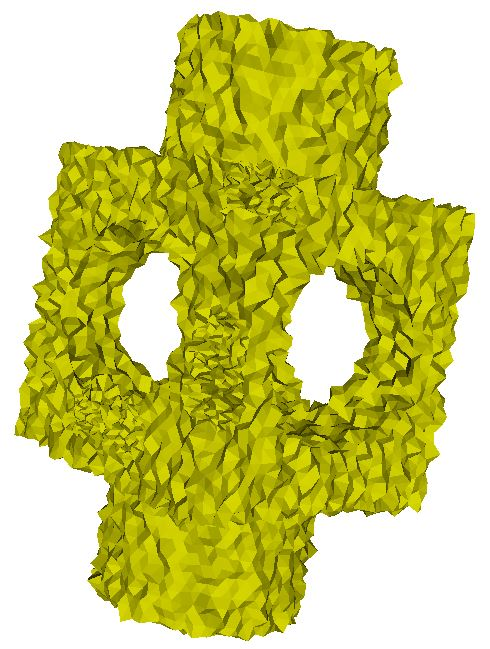
\includegraphics[width = 1.8cm]{results/block_Noisy.jpg}}
%\subfigure
%{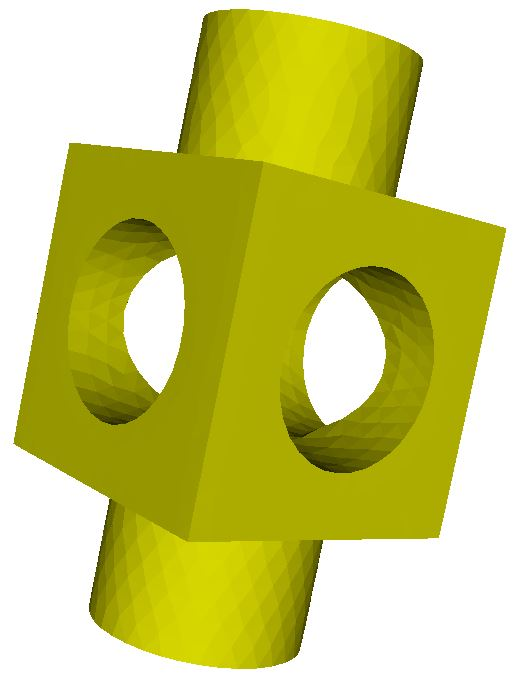
\includegraphics[width = 1.8cm]{results/block_Original.jpg}}
%\subfigure
%{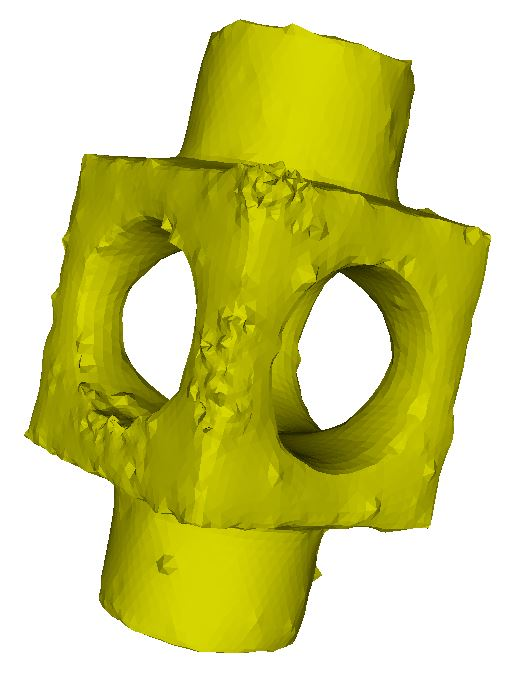
\includegraphics[width = 1.8cm]{results/block_FDCO03.jpg}}
%\subfigure
%{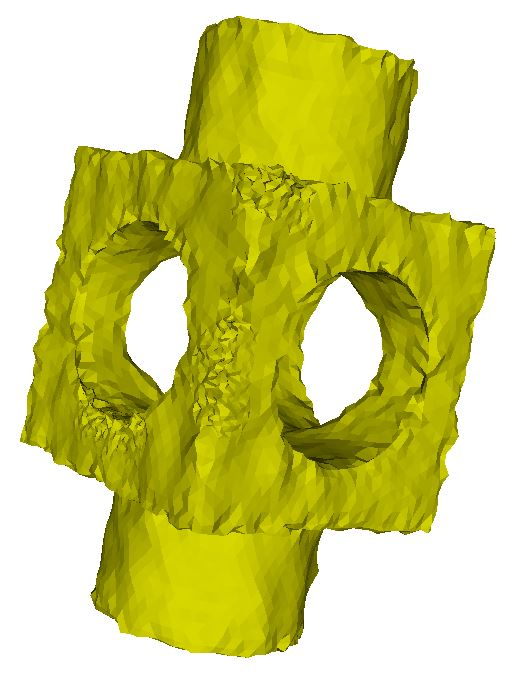
\includegraphics[width = 1.8cm]{results/block_JDD03.jpg}}
%\subfigure
%{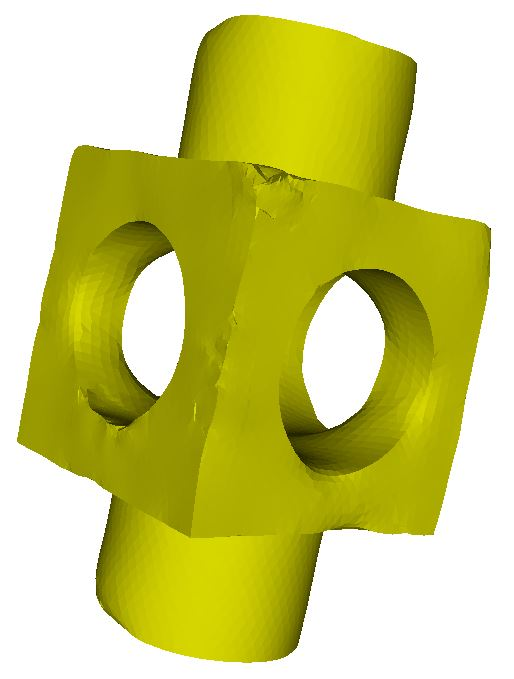
\includegraphics[width = 1.8cm]{results/block_SRML07.jpg}}
%\subfigure
%{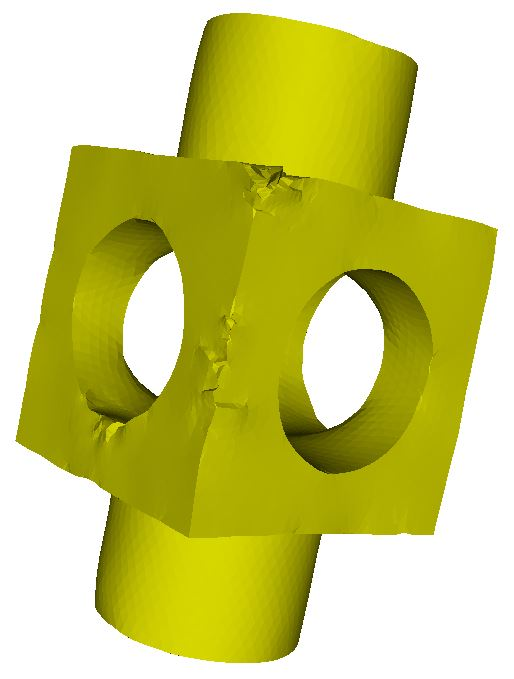
\includegraphics[width = 1.8cm]{results/block_ZFAT11local.jpg}}
%\subfigure
%{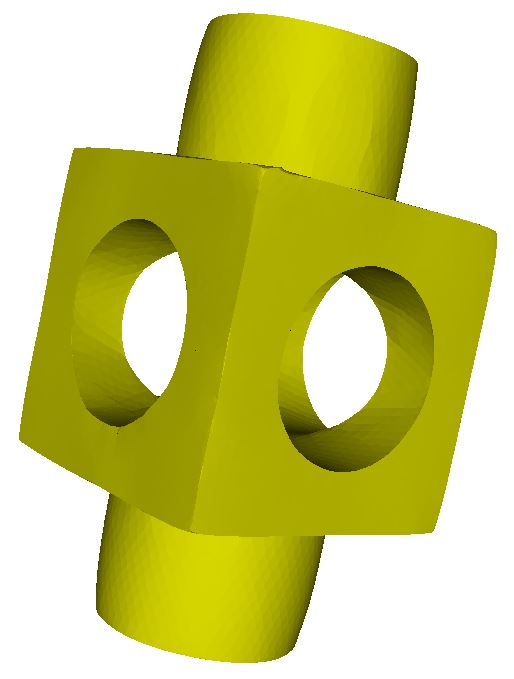
\includegraphics[width = 1.8cm]{results/block_HS13.jpg}}
%\subfigure
%{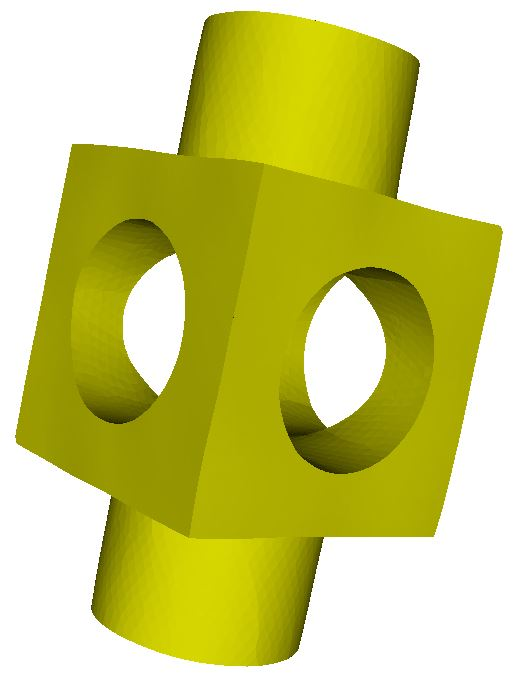
\includegraphics[width = 1.8cm]{results/block_PG15.jpg}}
%\subfigure
%{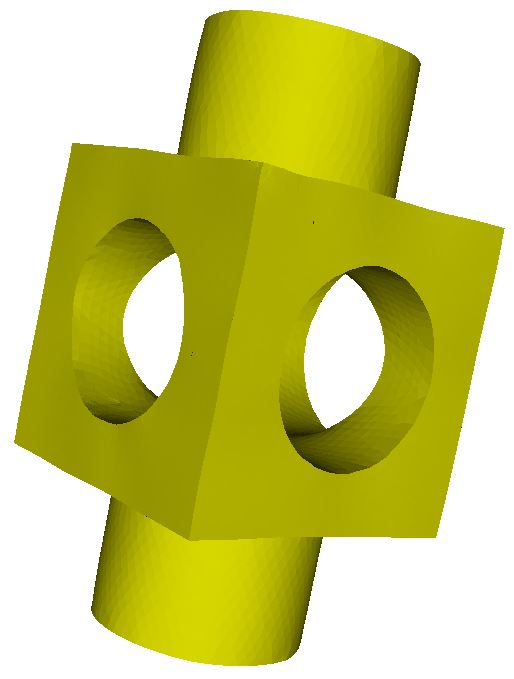
\includegraphics[width = 1.8cm]{results/block_our.jpg}}
%\\
%\vspace{-1.2mm}
%
%\subfigure
%{\includegraphics[width = 1.8cm]{results/twelve_Noisy.jpg}}
%\subfigure
%{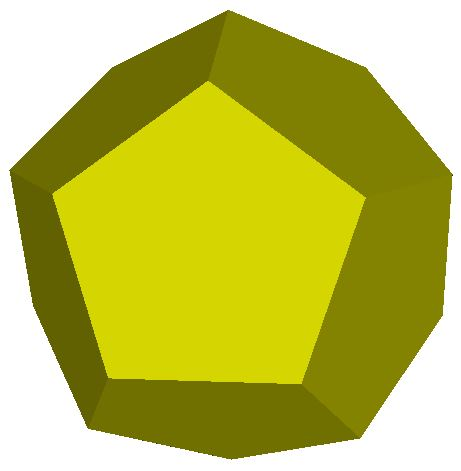
\includegraphics[width = 1.8cm]{results/twelve_Original.jpg}}
%\subfigure
%{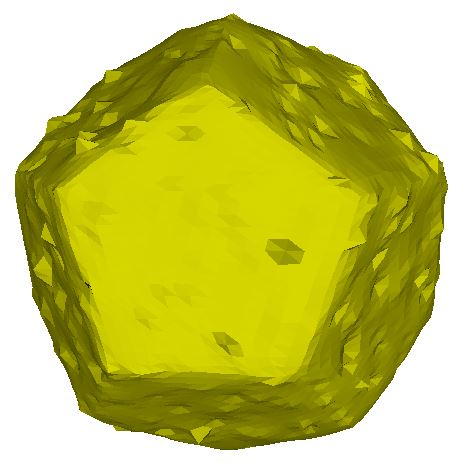
\includegraphics[width = 1.8cm]{results/twelve_FDCO03.jpg}}
%\subfigure
%{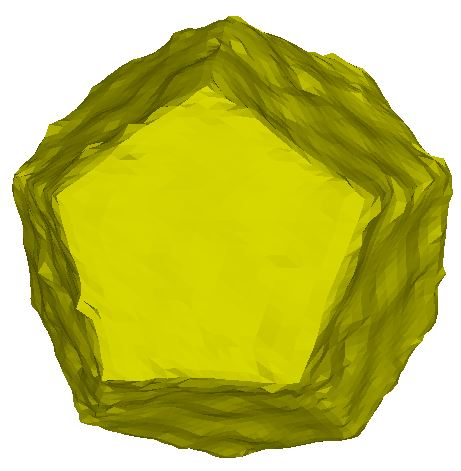
\includegraphics[width = 1.8cm]{results/twelve_JDD03.jpg}}
%\subfigure
%{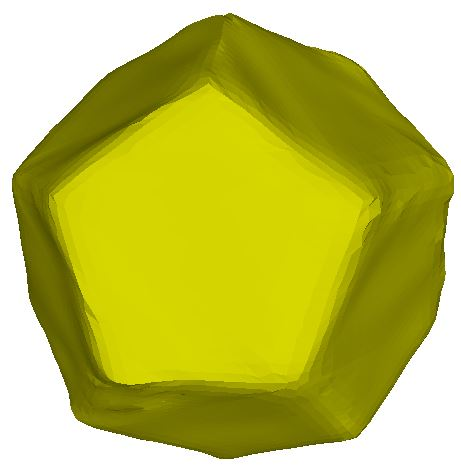
\includegraphics[width = 1.8cm]{results/twelve_SRML07.jpg}}
%\subfigure
%{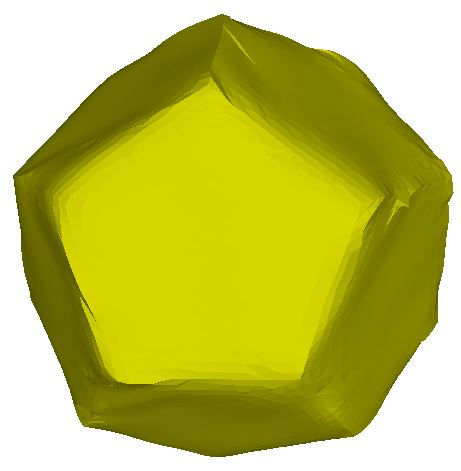
\includegraphics[width = 1.8cm]{results/twelve_ZFAT11local.jpg}}
%\subfigure
%{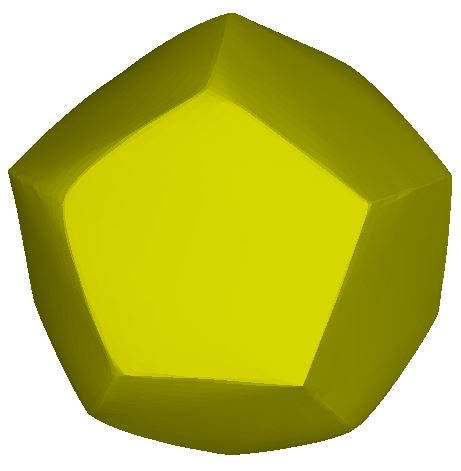
\includegraphics[width = 1.8cm]{results/twelve_HS13.jpg}}
%\subfigure
%{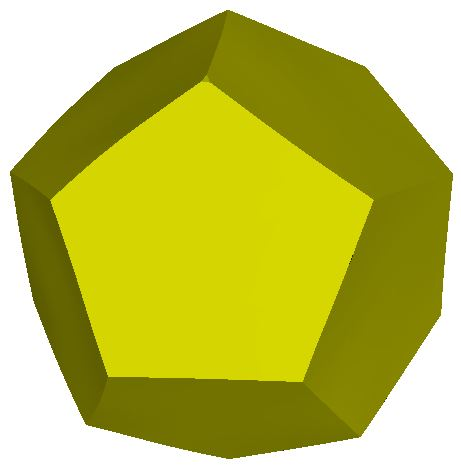
\includegraphics[width = 1.8cm]{results/twelve_PG15.jpg}}
%\subfigure
%{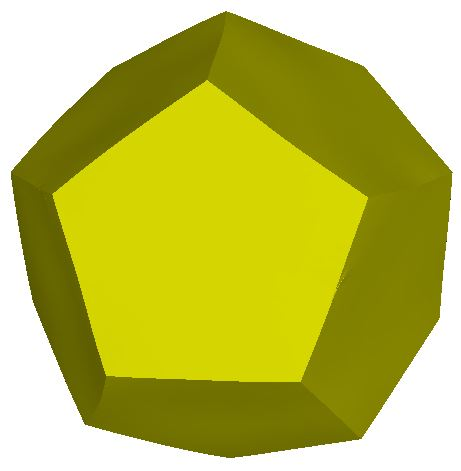
\includegraphics[width = 1.8cm]{results/twelve_our.jpg}}
%\caption{ Comparisons with other methods on synthetic meshes.}
%\label{Fig:special}
%\end{figure*}

















